% !TEX root = ../main.tex
\subsection{DIS plots in $v_z$ bins}
\label{20.04::dis_vz_plots}
    In Section \ref{14.31::phase_space_study}, we presented the acceptance-corrected DIS variables separated into $v_z$ bins.
    In this Appendix, we provide the same distributions without applying the acceptance correction.
    The statistics are considerably lower in $v_z$ bins characterised by low acceptance, such as $v_z > 10$ cm.
    This effect is more pronounced for the hadronic variables, as one would expect.
    Moreover, the correction noticeably alters the shape of certain distributions, bringing them closer to the expected theoretical behaviour.
    A clear illustration of this can be observed in the disparity of $Q^2$ depicted in Figures \ref{fig::14.31::q2_vz} and \ref{fig::20.04::q2_vz}, as well as in the dissimilarity of $z_h$ demonstrated in Figures \ref{fig::14.31::zh_211_vz} and \ref{fig::20.04::zh_211_vz}.

    % Q2.
    \begin{figure}
        \centering
        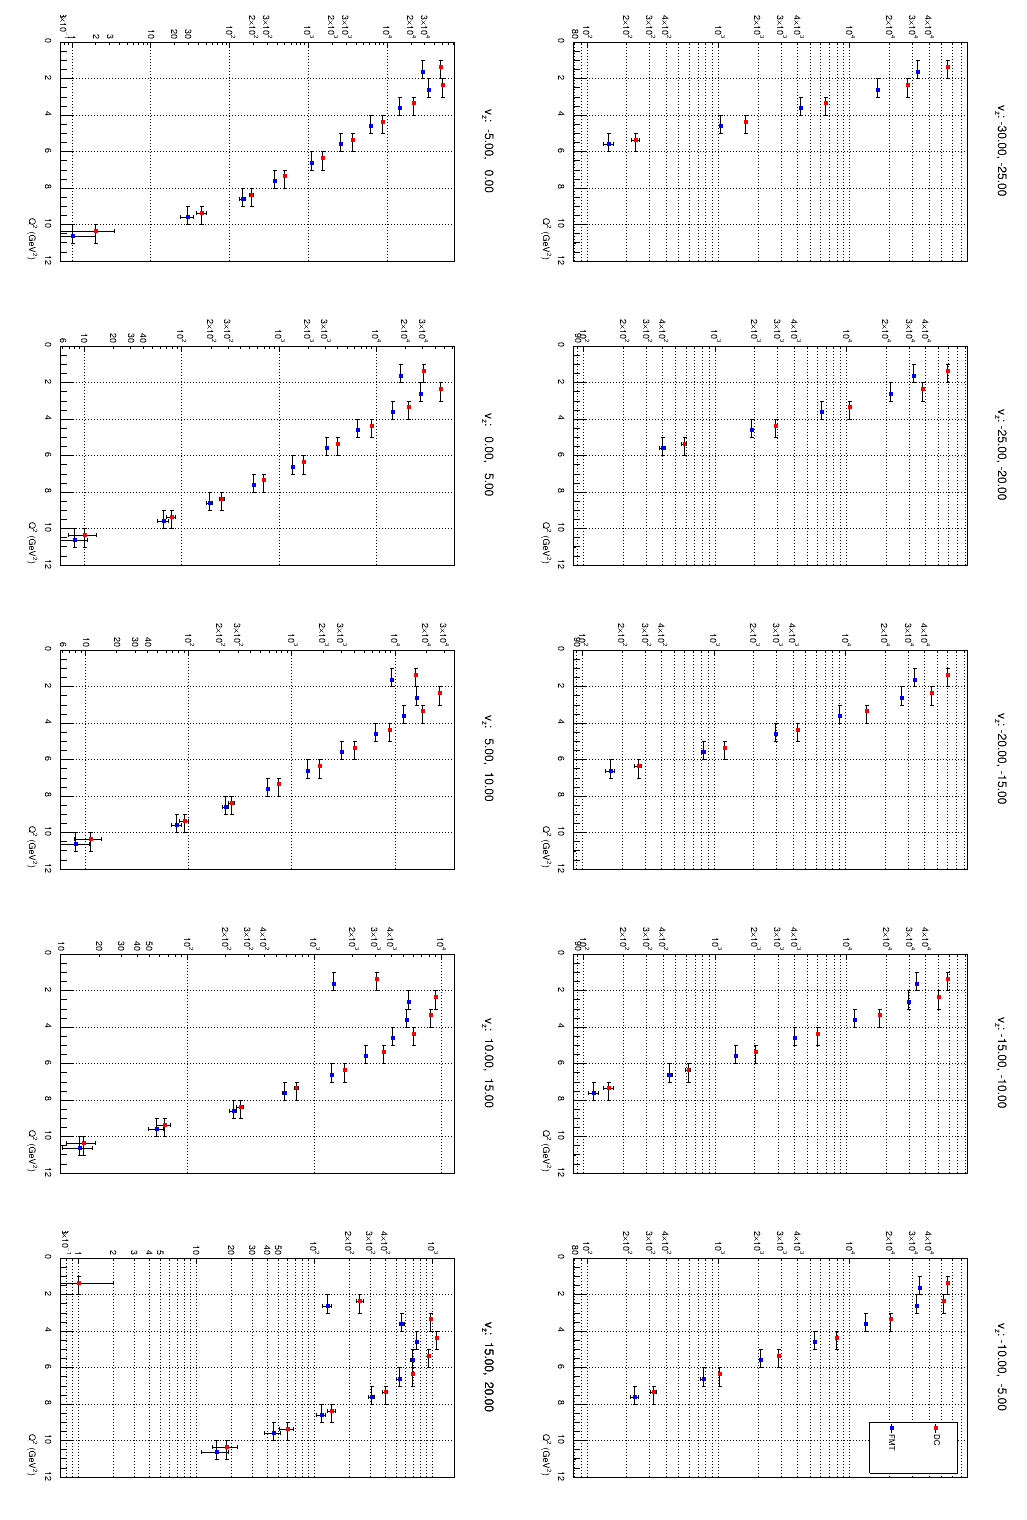
\includegraphics[width=\textwidth]{04q2_vz.png}
        \caption[$Q^2$ separated in $v_z$ bins]
        {$Q^2$ detected by DC and FMT, separated in $v_z$ bins.
        Run 12016.
        The bin markers are slightly shifted in $x$ to improve legibility.}
        \floatfoot{Source: Own elaboration, using the \href{https://github.com/bleaktwig/clas12-rge-analysis}{clas12-rge-analysis} software.}
        \label{fig::20.04::q2_vz}
    \end{figure}

    % nu.
    \begin{figure}
        \centering
        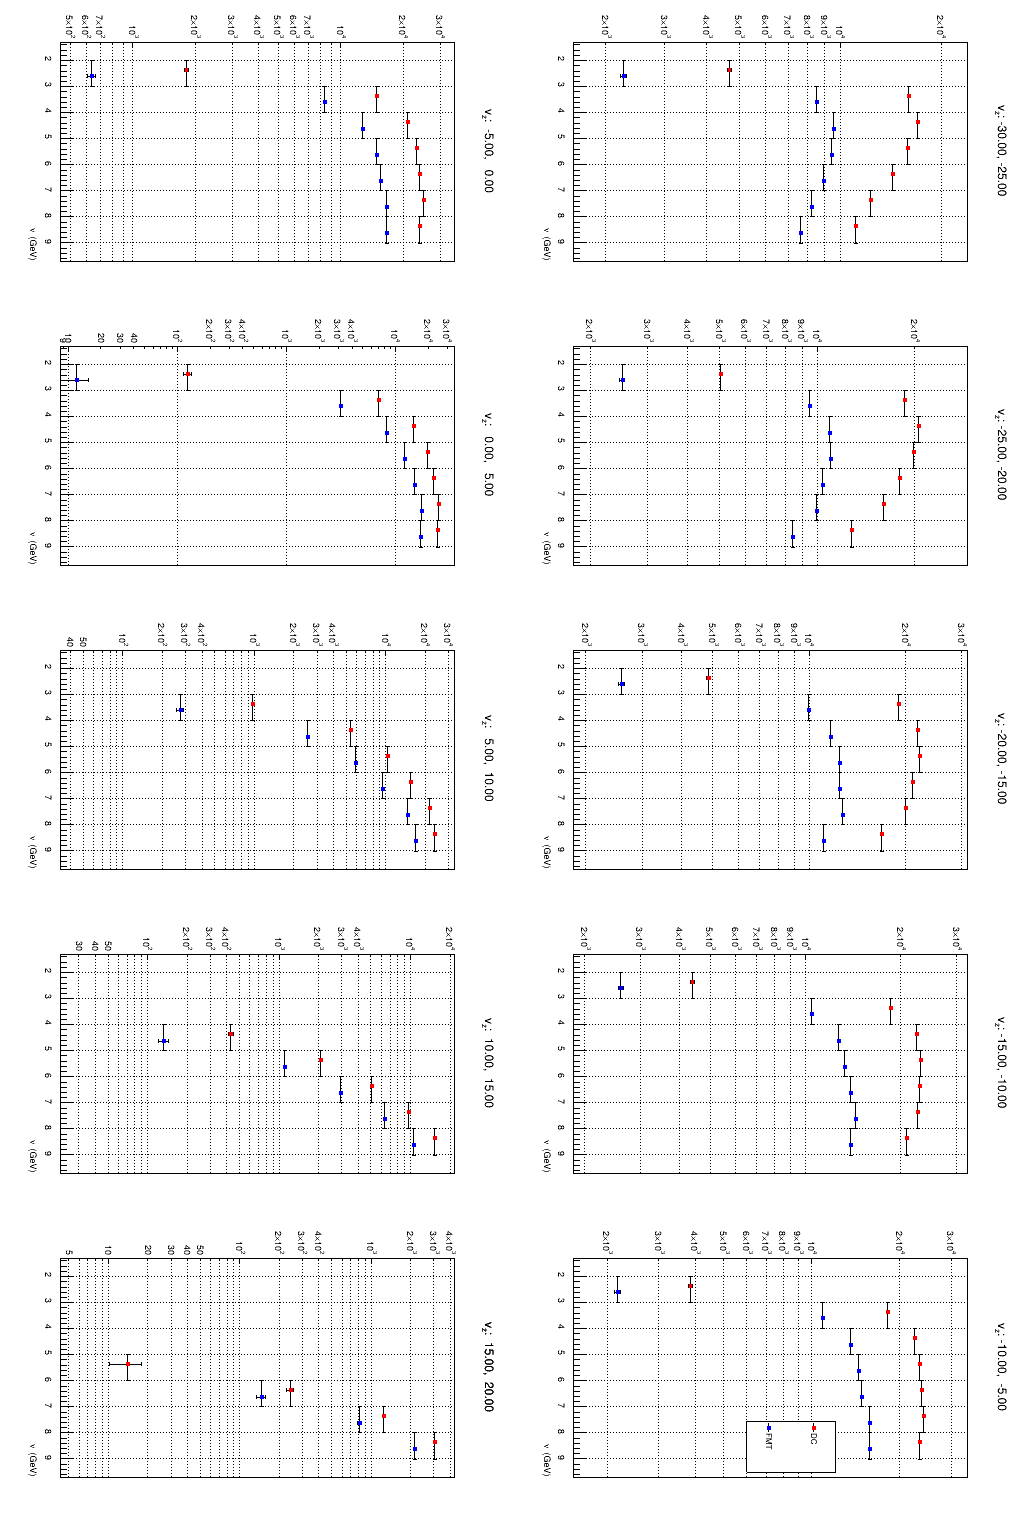
\includegraphics[width=\textwidth]{04nu_vz.png}
        \caption[$\nu$ separated in $v_z$ bins]
        {$\nu$ detected by DC and FMT, separated in $v_z$ bins.
        Run 12016.
        The bin markers are slightly shifted in $x$ to improve legibility.}
        \floatfoot{Source: Own elaboration, using the \href{https://github.com/bleaktwig/clas12-rge-analysis}{clas12-rge-analysis} software.}
        \label{fig::20.04::nu_vz}
    \end{figure}

    % zh.
    \begin{figure}
        \centering
        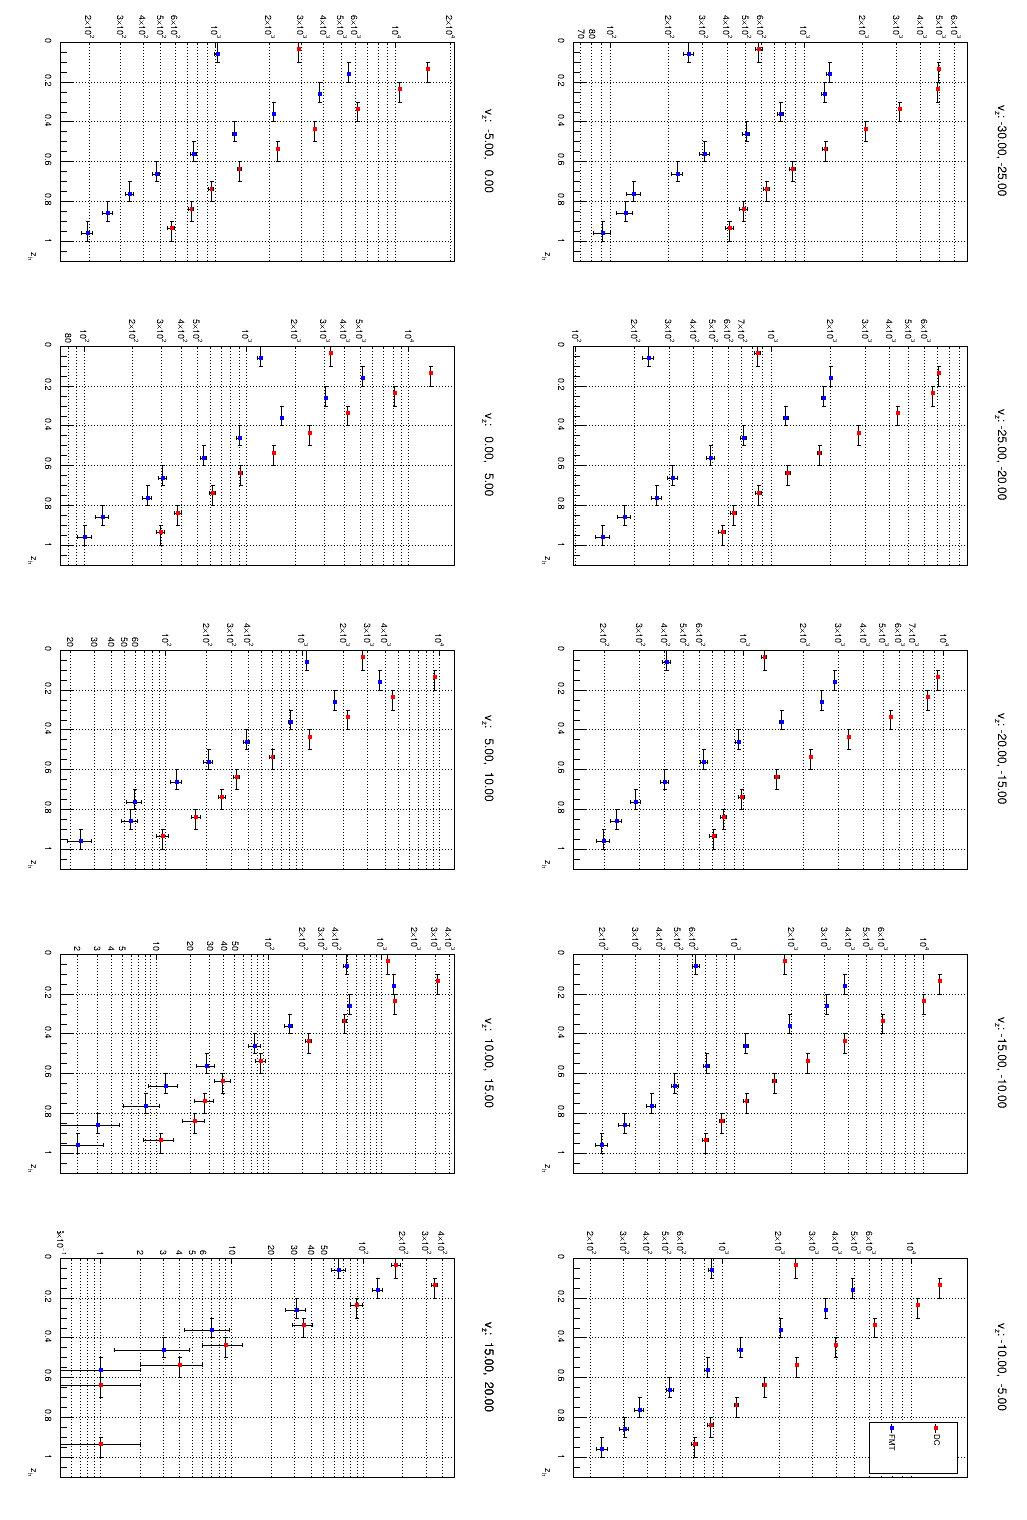
\includegraphics[width=\textwidth]{04zh_vz_211.png}
        \caption[$z_h$ for $e^-\pi^+$ separated in $v_z$ bins]
        {$z_h$ for $e^-\pi^+$ detected by DC and FMT, separated in $v_z$ bins.
        Run 12016.
        The bin markers are slightly shifted in $x$ to improve legibility.}
        \floatfoot{Source: Own elaboration, using the \href{https://github.com/bleaktwig/clas12-rge-analysis}{clas12-rge-analysis} software.}
        \label{fig::20.04::zh_211_vz}
    \end{figure}

    \begin{figure}
        \centering
        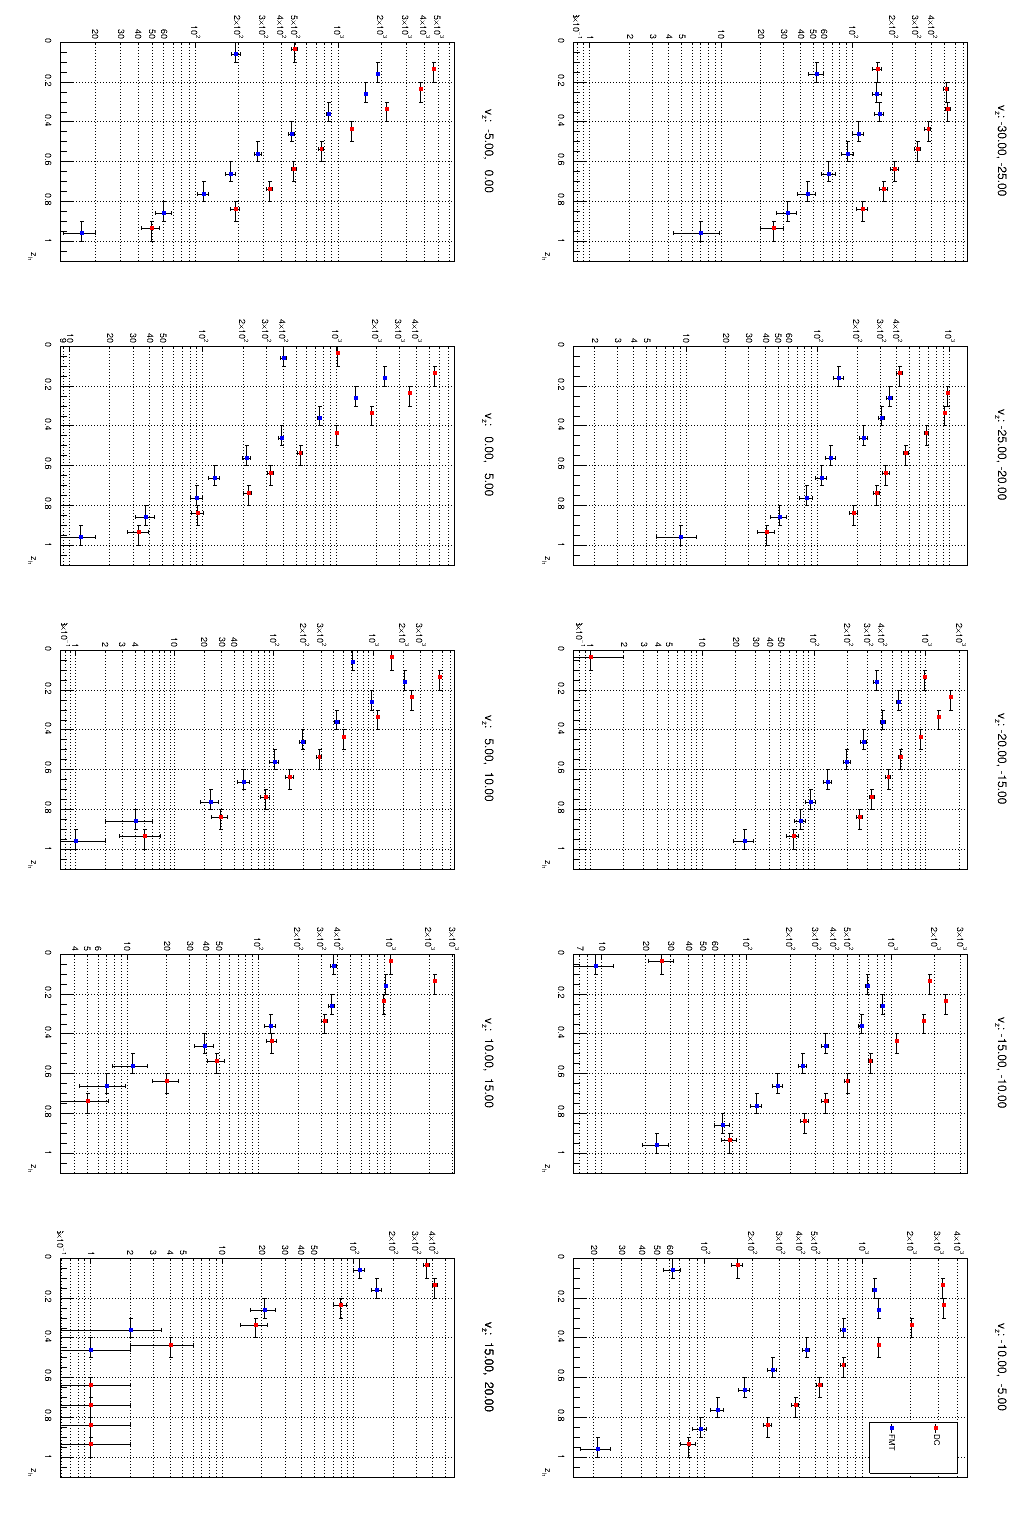
\includegraphics[width=\textwidth]{04zh_vz_-211.png}
        \caption[$z_h$ for $e^-\pi^-$ separated in $v_z$ bins]
        {$z_h$ for $e^-\pi^-$ detected by DC and FMT, separated in $v_z$ bins.
        Run 12016.
        The bin markers are slightly shifted in $x$ to improve legibility.}
        \floatfoot{Source: Own elaboration, using the \href{https://github.com/bleaktwig/clas12-rge-analysis}{clas12-rge-analysis} software.}
        \label{fig::20.04::zh_-211_vz}
    \end{figure}

    % pt2.
    \begin{figure}
        \centering
        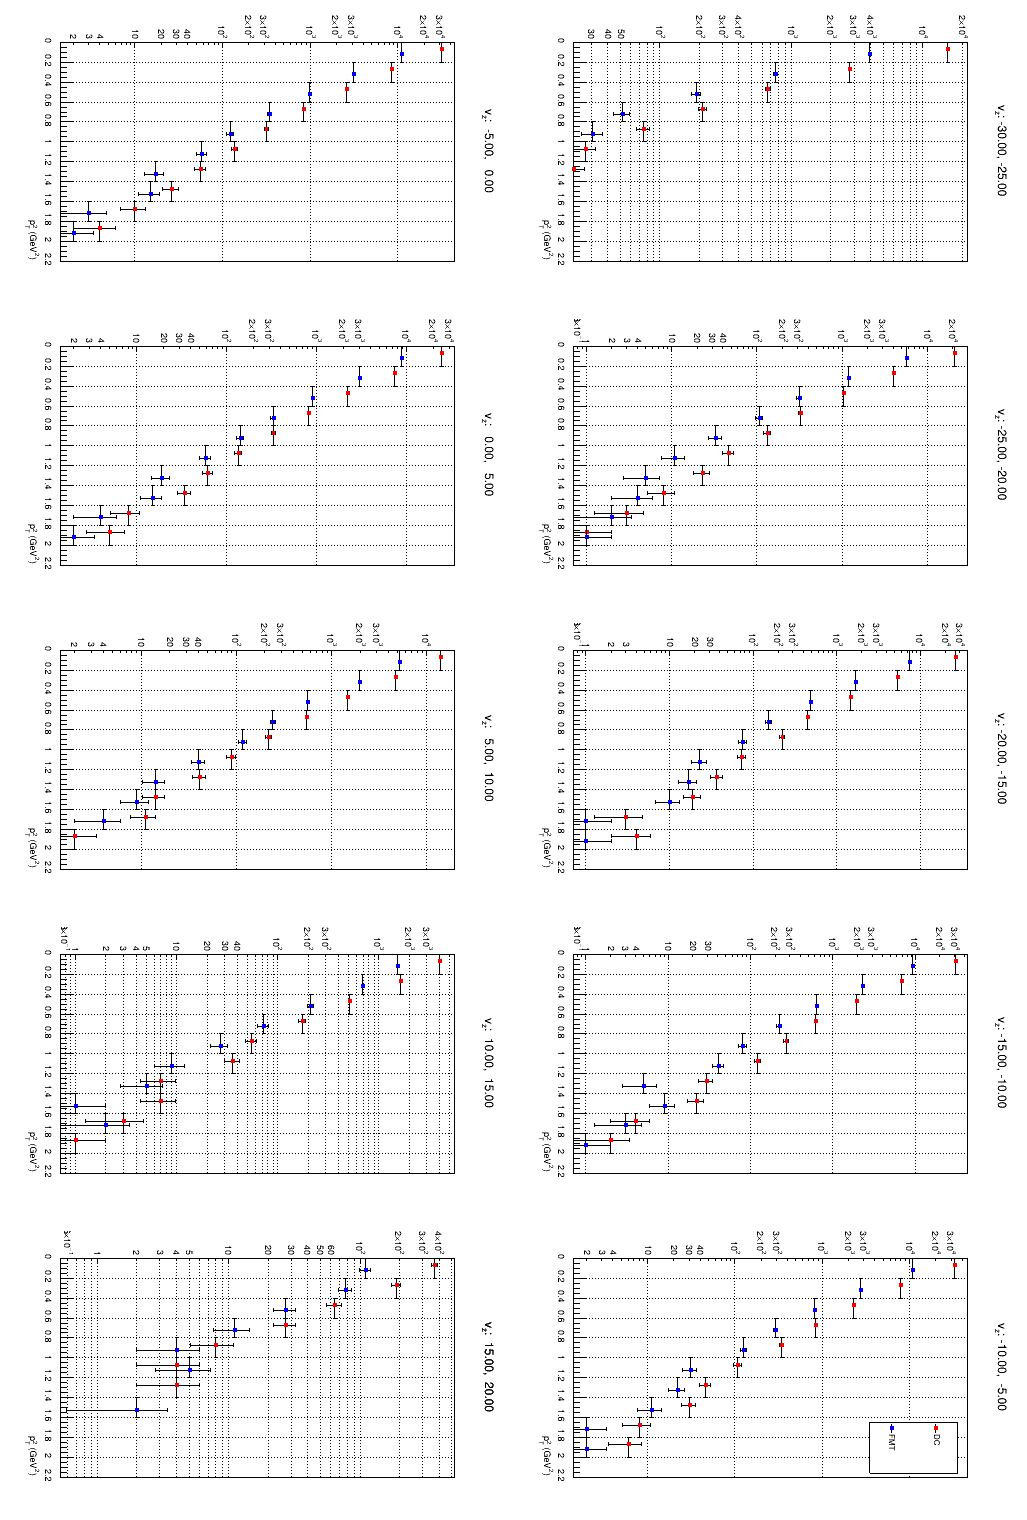
\includegraphics[width=\textwidth]{04pt2_vz_211.png}
        \caption[$p_T^2$ for $e^-\pi^+$ separated in $v_z$ bins]
        {$p_T^2$ for $e^-\pi^+$ detected by DC and FMT, separated in $v_z$ bins.
        Run 12016.
        The bin markers are slightly shifted in $x$ to improve legibility.}
        \floatfoot{Source: Own elaboration, using the \href{https://github.com/bleaktwig/clas12-rge-analysis}{clas12-rge-analysis} software.}
        \label{fig::20.04::pt2_211_vz}
    \end{figure}

    \begin{figure}
        \centering
        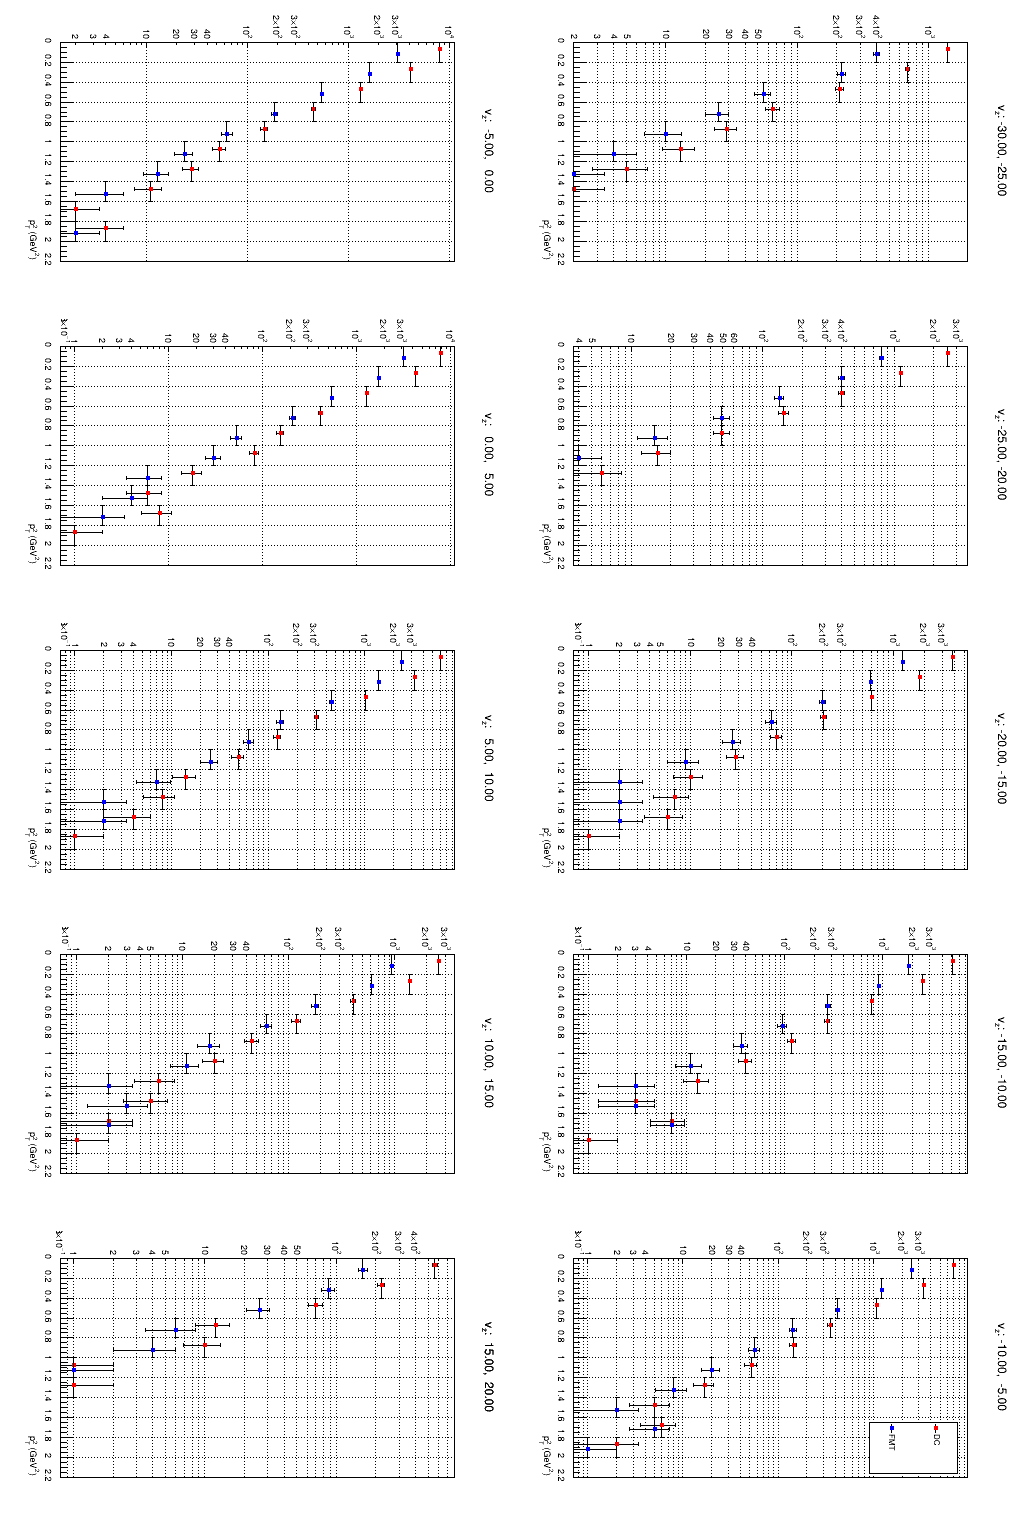
\includegraphics[width=\textwidth]{04pt2_vz_-211.png}
        \caption[$p_T^2$ for $e^-\pi^-$ separated in $v_z$ bins]
        {$p_T^2$ for $e^-\pi^-$ detected by DC and FMT, separated in $v_z$ bins.
        Run 12016.
        The bin markers are slightly shifted in $x$ to improve legibility.}
        \floatfoot{Source: Own elaboration, using the \href{https://github.com/bleaktwig/clas12-rge-analysis}{clas12-rge-analysis} software.}
        \label{fig::20.04::pt2_-211_vz}
    \end{figure}

    % phipq.
    \begin{figure}
        \centering
        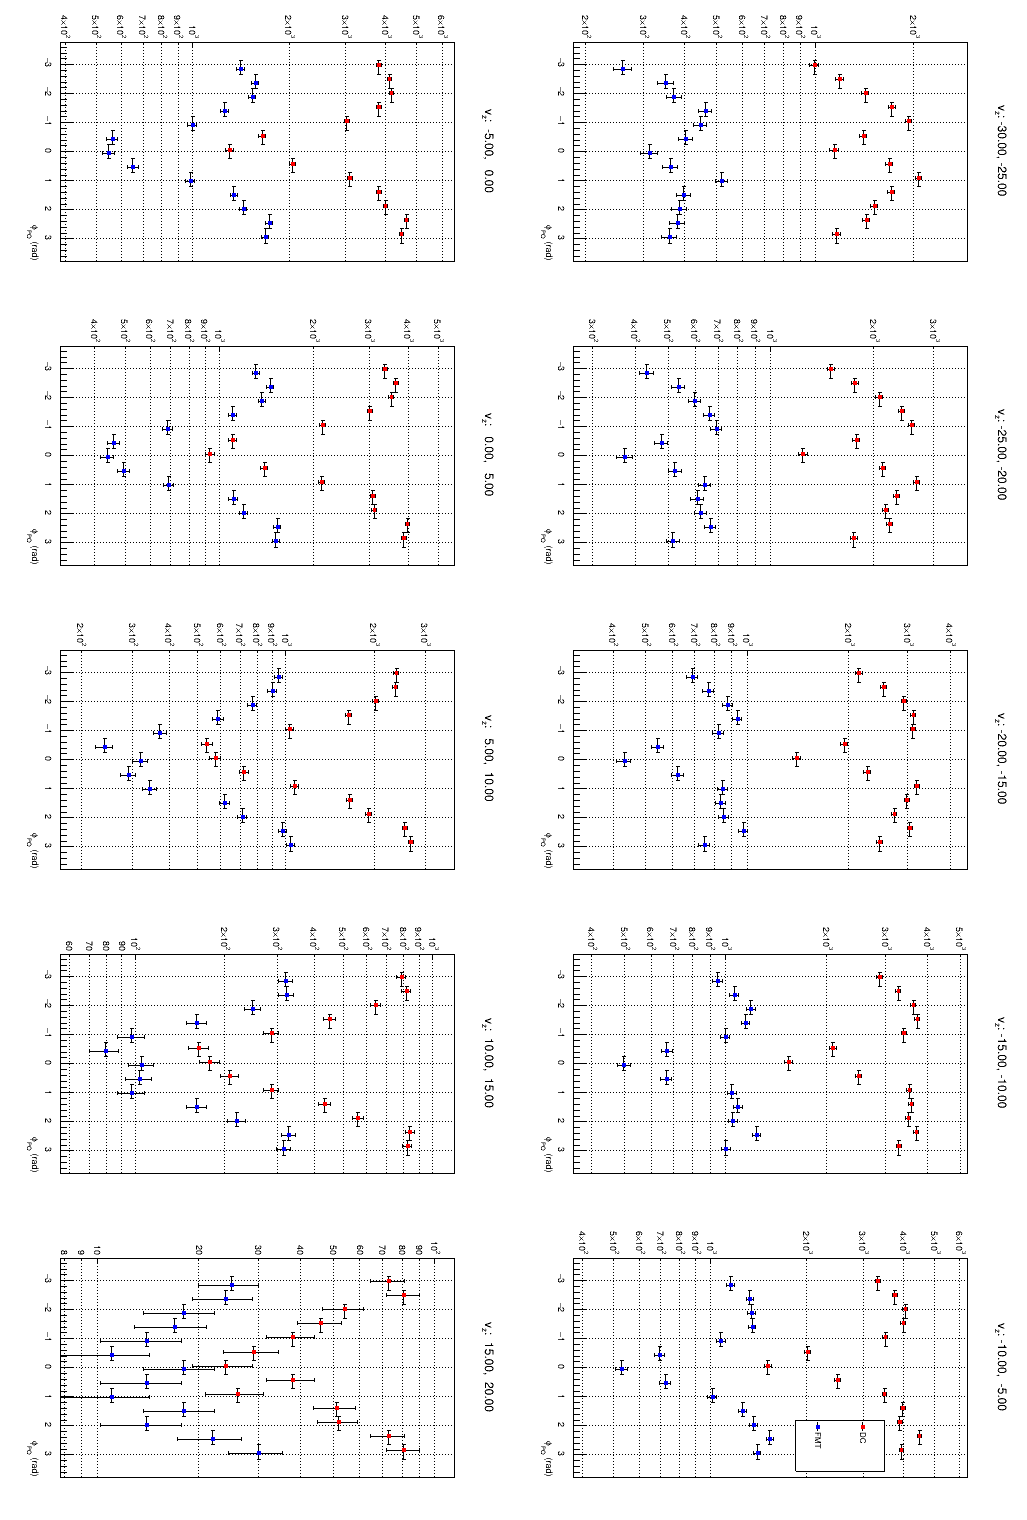
\includegraphics[width=\textwidth]{04phipq_vz_211.png}
        \caption[$\phi_{PQ}$ for $e^-\pi^+$ separated in $v_z$ bins]
        {$\phi_{PQ}$ for $e^-\pi^+$ detected by DC and FMT, separated in $v_z$ bins.
        Run 12016.
        The bin markers are slightly shifted in $x$ to improve legibility.}
        \floatfoot{Source: Own elaboration, using the \href{https://github.com/bleaktwig/clas12-rge-analysis}{clas12-rge-analysis} software.}
        \label{fig::20.04::phipq_211_vz}
    \end{figure}

    \begin{figure}
        \centering
        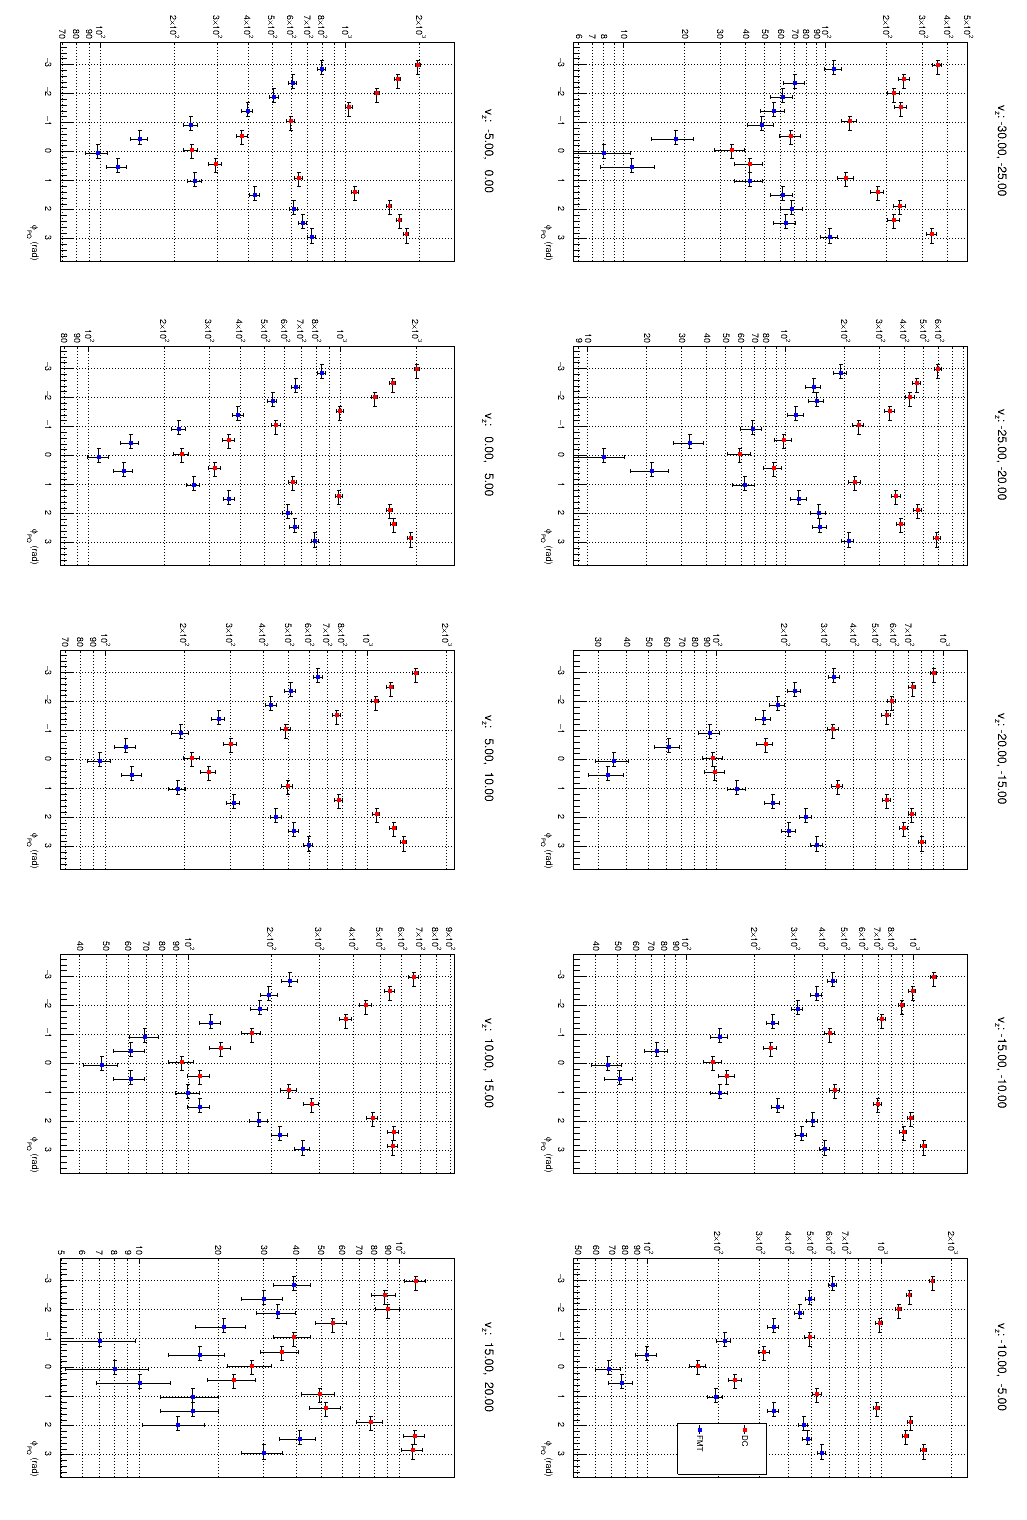
\includegraphics[width=\textwidth]{04phipq_vz_-211.png}
        \caption[$\phi_{PQ}$ for $e^-\pi^-$ separated in $v_z$ bins]
        {$\phi_{PQ}$ for $e^-\pi^-$ detected by DC and FMT, separated in $v_z$ bins.
        Run 12016.
        The bin markers are slightly shifted in $x$ to improve legibility.}
        \floatfoot{Source: Own elaboration, using the \href{https://github.com/bleaktwig/clas12-rge-analysis}{clas12-rge-analysis} software.}
        \label{fig::20.04::phipq_-211_vz}
    \end{figure}

    % \pagebreak
